\section{Projeto do filtro}
\label{sec:metodologia}

\subsection{De onde saem as especificações}

O enunciado já entrega os números principais, mas vale dizer de onde cada um vem, porque nem todos estão na tabela de dados.

A faixa de passagem vai até $100$~kHz simplesmente porque é essa a banda que o canal útil ocupa ($\pm 100$~kHz em torno de zero). A faixa de rejeição começa em $200$~kHz porque é ali que está o canal vizinho, o primeiro sinal que não queremos deixar passar. Entre um e outro sobra uma faixa de transição de $100$~kHz, que é o espaço que o filtro tem para sair do ganho $1$ e chegar perto de zero.

Como o projeto é feito em tempo discreto, as frequências precisam ser normalizadas em relação à taxa de amostragem. Usando $\omega = 2\pi f / F_s$:

\begin{equation}
\omega_p = 2\pi\frac{100}{1920} = 0{,}3272 \ \mathrm{rad/amostra}, \qquad
\omega_s = 2\pi\frac{200}{1920} = 0{,}6545 \ \mathrm{rad/amostra},
\end{equation}

\begin{equation}
\Delta\omega = \omega_s - \omega_p = 0{,}3272 \ \mathrm{rad/amostra}.
\end{equation}

As tolerâncias de amplitude saem das duas exigências em decibéis. Na passagem, o ganho pode variar $0{,}1$~dB de pico a pico, o que dá

\begin{equation}
20\log_{10}\frac{1+\delta_1}{1-\delta_1} = 0{,}1 \ \mathrm{dB}
\quad \Longrightarrow \quad
\delta_1 = 0{,}0058 ,
\end{equation}

e na rejeição a atenuação de $60$~dB corresponde a

\begin{equation}
\delta_2 = 10^{-60/20} = 0{,}001 .
\end{equation}

\subsection{Uma especificação que não está na tabela}

Aqui aparece o detalhe mais importante do projeto, e ele não está escrito na lista de dados fornecidos.

O critério de aprovação pede que o interferente de $450$~kHz, depois de dobrar sobre o canal, fique $60$~dB \textbf{abaixo} do canal útil. Só que, no sinal de teste, esse interferente tem amplitude $6$ enquanto o canal útil tem amplitude $1$. Ou seja, ele já chega

\begin{equation}
20\log_{10}(6) = 15{,}56 \ \mathrm{dB}
\end{equation}

\textbf{acima} do sinal que queremos. Para ele terminar $60$~dB abaixo, o filtro não pode atenuar $60$~dB — precisa atenuar

\begin{equation}
A = 60 + 15{,}56 = 75{,}56 \ \mathrm{dB}
\label{eq:atenuacao-projeto}
\end{equation}

na região de $450$~kHz. Esse é o valor que realmente dimensiona o filtro. Projetando com os $60$~dB nominais, o filtro sai com $71$ coeficientes e o interferente termina em $-57{,}4$~dB relativos ao útil, ou seja, $2{,}6$~dB acima do limite: reprovaria no critério. Por isso a atenuação de projeto adotada foi a da Equação~\eqref{eq:atenuacao-projeto}.

Vale notar que o canal adjacente, apesar de entrar ainda mais forte ($20\log_{10}(8) = 18{,}06$~dB acima do útil), é menos exigente: ele fica fora do canal depois da decimação, então basta a rejeição de $60$~dB pedida no enunciado.

\subsection{Por que um FIR com janela de Kaiser}

O bloco seguinte da cadeia é um classificador que decide olhando a constelação I/Q, ou seja, olhando amplitude e fase dos símbolos. Se o filtro atrasar cada frequência de um jeito diferente, os pontos da constelação saem do lugar e se espalham, e o classificador erra. Um filtro FIR com coeficientes simétricos resolve isso de graça: a fase dele é uma reta e o atraso é o mesmo para todas as frequências. O sinal sai apenas deslocado no tempo, sem deformação.

Um filtro IIR teria ordem bem menor, mas a fase dele não é linear, e ainda por cima ele não se decompõe em forma polifásica (o motivo está detalhado na Seção~\ref{sec:conceitual}). Por isso a escolha foi o FIR.

Entre os métodos de janelamento, a janela de Kaiser é a única com um parâmetro ajustável. As janelas fixas entregam sempre a mesma atenuação — retangular $21$~dB, Hanning $44$~dB, Hamming $53$~dB, Blackman $74$~dB — então ou não atendem o que precisamos, ou atendem com sobra e cobram coeficientes a mais por isso. Na Kaiser, o parâmetro $\beta$ é calculado a partir da atenuação exigida, e o filtro sai com o menor comprimento possível dentro do método.

\subsection{As contas do projeto}

O procedimento seguido é o dos slides da disciplina. Com $\delta = \delta_2$ e a atenuação de projeto da Equação~\eqref{eq:atenuacao-projeto}, calcula-se primeiro o parâmetro da janela, que para $A > 50$~dB vale

\begin{equation}
\beta = 0{,}1102\,(A - 8{,}7) = 7{,}3683 ,
\end{equation}

e depois o comprimento do filtro, que depende da largura da faixa de transição:

\begin{equation}
M \simeq \frac{A - 7{,}95}{2{,}285\,\Delta\omega} + 1 = 91{,}42 \quad \Longrightarrow \quad M = 93 .
\end{equation}

O valor foi arredondado para cima e forçado a ímpar, para que o atraso

\begin{equation}
\alpha = \frac{M-1}{2} = 46 \ \mathrm{amostras}
\end{equation}

seja um número inteiro de amostras (filtro de Tipo I).

A frequência de corte do filtro ideal é colocada no meio da faixa de transição,

\begin{equation}
\omega_c = \frac{\omega_p + \omega_s}{2} = 0{,}4909 \ \mathrm{rad/amostra} \qquad (f_c = 150 \ \mathrm{kHz}),
\end{equation}

e a resposta ao impulso final é o produto do passa-baixas ideal pela janela:

\begin{equation}
h(n) = \underbrace{\frac{\mathrm{sen}\big(\omega_c(n-\alpha)\big)}{\pi(n-\alpha)}}_{\text{filtro ideal}}
\cdot
\underbrace{\frac{I_0\!\left[\beta\sqrt{1 - \left(1 - \frac{2n}{M-1}\right)^2}\right]}{I_0[\beta]}}_{\text{janela de Kaiser}},
\qquad 0 \le n \le M-1 .
\label{eq:hn}
\end{equation}

A função $I_0$ é a Bessel modificada de primeira espécie e ordem zero, calculada pela série

\begin{equation}
I_0(x) = 1 + \sum_{k=1}^{\infty}\left[\frac{(x/2)^k}{k!}\right]^2 ,
\end{equation}

que converge rápido: para $\beta = 7{,}37$ os termos já caem abaixo de $10^{-11}$ por volta do vigésimo, então uma soma com poucas dezenas de termos dá precisão de máquina.

A Figura~\ref{fig:projeto} mostra o resultado dessas contas. No canto superior esquerdo está a janela, que vale quase zero nas bordas e $1$ no centro. No canto superior direito aparece o filtro ideal (tracejado) e o filtro final (cheio): a janela vai suavizando as oscilações da ponta, e é isso que derruba os lóbulos laterais. Embaixo, à esquerda, a resposta em frequência já pronta contra a máscara de especificação, e à direita um zoom da faixa de passagem mostrando que a ondulação é muito menor que o limite.

\begin{figure}[htb]
\centering
\caption{Etapas do projeto: janela de Kaiser, resposta ao impulso e verificação contra a máscara de especificação.}
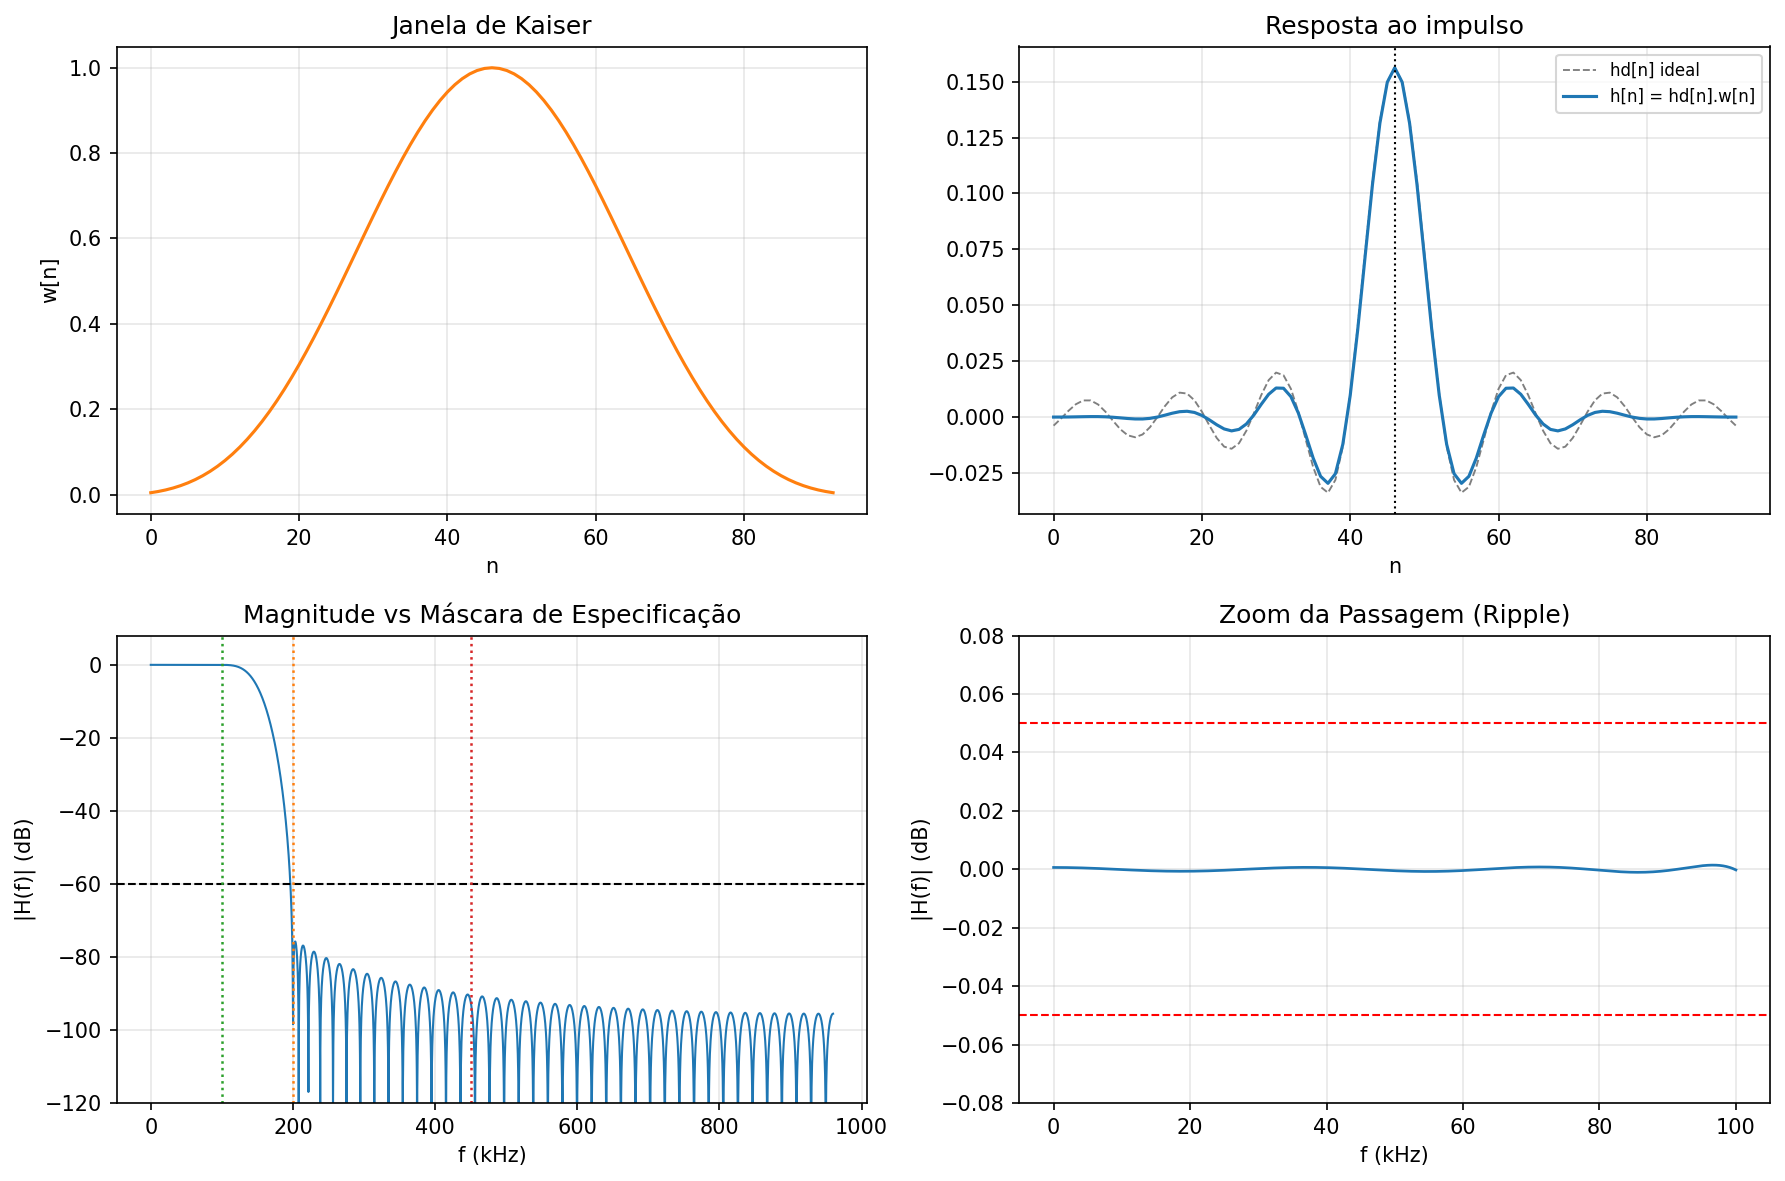
\includegraphics[width=\linewidth]{Imagens/fig02_projeto_filtro.png}
\label{fig:projeto}
\fonte{Autoria própria.}
\end{figure}

Os parâmetros obtidos estão reunidos na Tabela~\ref{tab:parametros}.

\begin{table}[htb]
\centering
\caption{Parâmetros do filtro projetado.}
\label{tab:parametros}
\begin{tabular}{ll}
\hline
\textbf{Parâmetro} & \textbf{Valor} \\
\hline
Tolerância de projeto $\delta$ & $0{,}001$ \\
Atenuação exigida pelo canal adjacente & $60{,}00$~dB \\
Atenuação exigida pelo interferente & $75{,}56$~dB \\
Atenuação de projeto $A$ & $75{,}56$~dB \\
Parâmetro da janela $\beta$ & $7{,}3683$ \\
Comprimento $M$ & $93$ coeficientes \\
Atraso $\alpha$ & $46$ amostras ($23{,}96$~$\mu$s) \\
Frequência de corte $f_c$ & $150$~kHz ($\omega_c = 0{,}4909$) \\
\hline
\end{tabular}
\fonte{Autoria própria.}
\end{table}
